% Read and consider:

% Read-Log-Update A Lightweight Synchronization Mechanism for Concurrent
% Programming Matveev, et al. SOSP 2015
% http://sigops.org/sosp/sosp15/current/2015-Monterey/printable/077-matveev.pdf

% In 3 to 4 pages:
% 1. Briefly outline how RLU works.
% 2. Explain the problem that RLU Deferring (Section 3.7) solves and give a
% pathological example scenario where RCU’s “synchronize” operation would have
% high overheads but RLU Deferral wouldnot.
% 3. Explain: can RLU Deferral result in linearizability violations?
% 4. Explain: does code using RLU Deferral in 3.7 meet the definition of being
% “lock-free”.

\begin{refsection}
\section{Questions from Ryan Stutsman}
\label{sec:member4}

\subsection*{Briefly outline how RLU works.}
\label{sec:member41}

The authors in~\cite{Matveev:2015:RLS:2815400.2815406} introduce
\emph{read-log-update} (RLU), a novel extension of \emph{read-copy-update}
(RCU)~\cite{McKenney}, a synchronization mechanism already embedded in the
Linux Kernel.
%
RLU is a synchronization mechanism for concurrent programming that allows
unsynchronized sequences of reads to execute concurrently with writes,
granting a significant gain in terms of performance for operations in many
data structures and applications.
%
The main difference between RCU and RLU is that, the latter overcomes the main
limitations of RCU by allowing concurrent reads with multiple writers.
%
RLU provides a framework to improve the performance of concurrent
data-structures usage by supporting:
\begin{itemize}
\item \emph{Unsynchronized traversals}: as the 90\% of the time is spent
  traversing (reading) data, the key to enhancing performance is to make these
  reads as efficient as possible without using any locks, memory fences or
  writes;
\item \emph{Multi-location atomic updates}: short atomic updates that can be
  applied to small sections of concurrent data structures in order to hide
  from the programmers the complexity of dealing with race condition.
\end{itemize}

\subsubsection*{RCU Description}
\label{sec:member411}
RCU is a synchronization mechanism that provides support for
\emph{unsynchronized traversal} but not multi-location atomic updates.
%
Indeed, RCU only supports single pointer updates making it really difficult to
program in non-trivial cases such as complex data-structures (e.g.\ trees, in
the Linux kernel is mainly used on variations of linked lists).
%
However, it is very efficient as there are no overheads for reads.

The main ideas behind the RCU mechanism are: (1) \emph{to modify objects} RCU
duplicates them and modifies the copies guaranteeing at the same time
unsynchronized reads; (2) \emph{to commit a modification} RCU uses a single
pointer update making the new copies of the objects reachable and the old
copies unreachable.
%
The pointers update needs to be atomic (happen all at once) this is sometime
very complex to obtain.

\paragraph*{Example:}

\begin{figure}[b]
  \vspace{-10pt}
  \begin{minipage}[b]{0.47\textwidth}
    \begin{flushleft}
      \centering
      \raisebox{10pt}{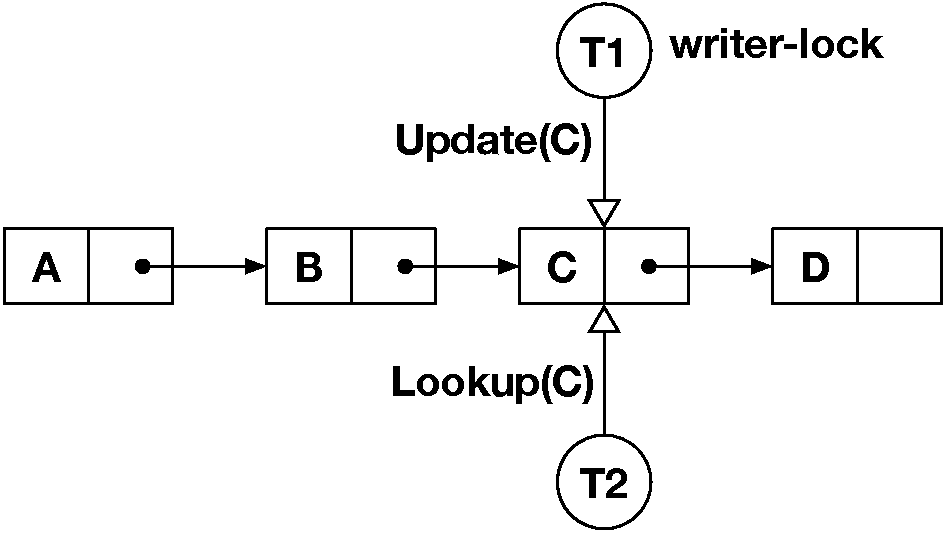
\includegraphics[width=0.9\textwidth]{figures/rcu_ex1}}
      \caption{Two threads access a list respectively to update and a lookup the
        node \emph{C}.}
      \label{fig:rcu_ex1}
    \end{flushleft}
  \end{minipage}
  \hfill
  \begin{minipage}[b]{0.47\textwidth}
    \begin{flushright}
      \centering
      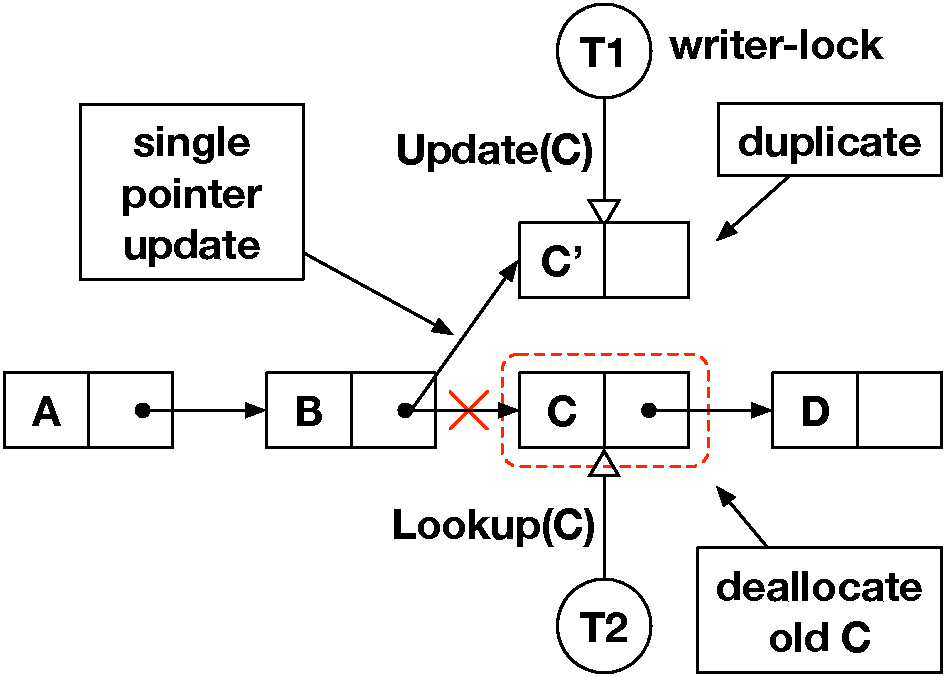
\includegraphics[width=0.9\textwidth]{figures/rcu_ex2}
      \caption{The writer \emph{T1} duplicates the node \emph{C} and performs the
        single pointer update.}
      \label{fig:rcu_ex2}
    \end{flushright}
  \end{minipage}
  \vspace{-10pt}
\end{figure}

Let us suppose that we have two threads that we want to access a linked list,
like the one in Figure~\ref{fig:rcu_ex1}.
%
The thread \emph{T1} wants to update the node \emph{C} while the thread
\emph{T2} concurrently wants to lookup for the node \emph{C}.
%
We then have a conflict between the two threads.
%
The thread \emph{T1} acquires a \emph{write-lock} and it starts to traverse
the list, at the same time the thread \emph{T2} starts looking for the node
\emph{C} traversing the list as well.
%
Let us assume that both threads reach the node \emph{C} at the same time, as
shown in Figure~\ref{fig:rcu_ex1}.
%
In order to avoid conflict, the thread \emph{T1} duplicates the node \emph{C}
(to \emph{C'}) and performs a single pointer update making \emph{C'} reachable
and \emph{C} unreachable, as illustrated in Figure~\ref{fig:rcu_ex2}.
%
The final operation consists in deallocating the old node \emph{C}.
%
Prior to deleting the node \emph{C}, the thread \emph{T1} needs to make sure
that no other threads are still reading it.
%
For this purpose, it waits for a \emph{grace period}, a time interval after
which it is safe to deallocate the object.

This example shows how RCU is able to perform a single pointer update.
%
However, applying RCU to more complex data structures or operations may result
in a less straightforward pointers update.
%
Let us suppose to have a linked list where a thread \emph{T1} wants to update
all the even nodes, as shown in Figure~\ref{fig:rcu_ex3}.
%
Thread \emph{T1} duplicates the node that it wants to update, and then it
needs to update their pointers.
%
With a single pointer update it is impossible to update both pointers at the
same time.
%
Therefore, thread \emph{T1}, for instance, updates first the pointer to the
node \emph{B'}.
%
If at the same time another thread \emph{T2} (Figure~\ref{fig:rcu_ex4}) tries
to lookup for all the even nodes, it will see an inconsistent mix of states
that would not happen in any serial execution on this data structure.
%
In order to find a solution to this problem, programmers must be able to see
this kind of race conditions and solve them manually using some
synchronization mechanism.
%
However, with more complex data structures (e.g.\ search tree, graph) solving
these race conditions may prove very difficult.

\begin{figure}
  \begin{minipage}[t]{0.47\textwidth}
    \begin{flushleft}
      \centering
      \raisebox{0pt}{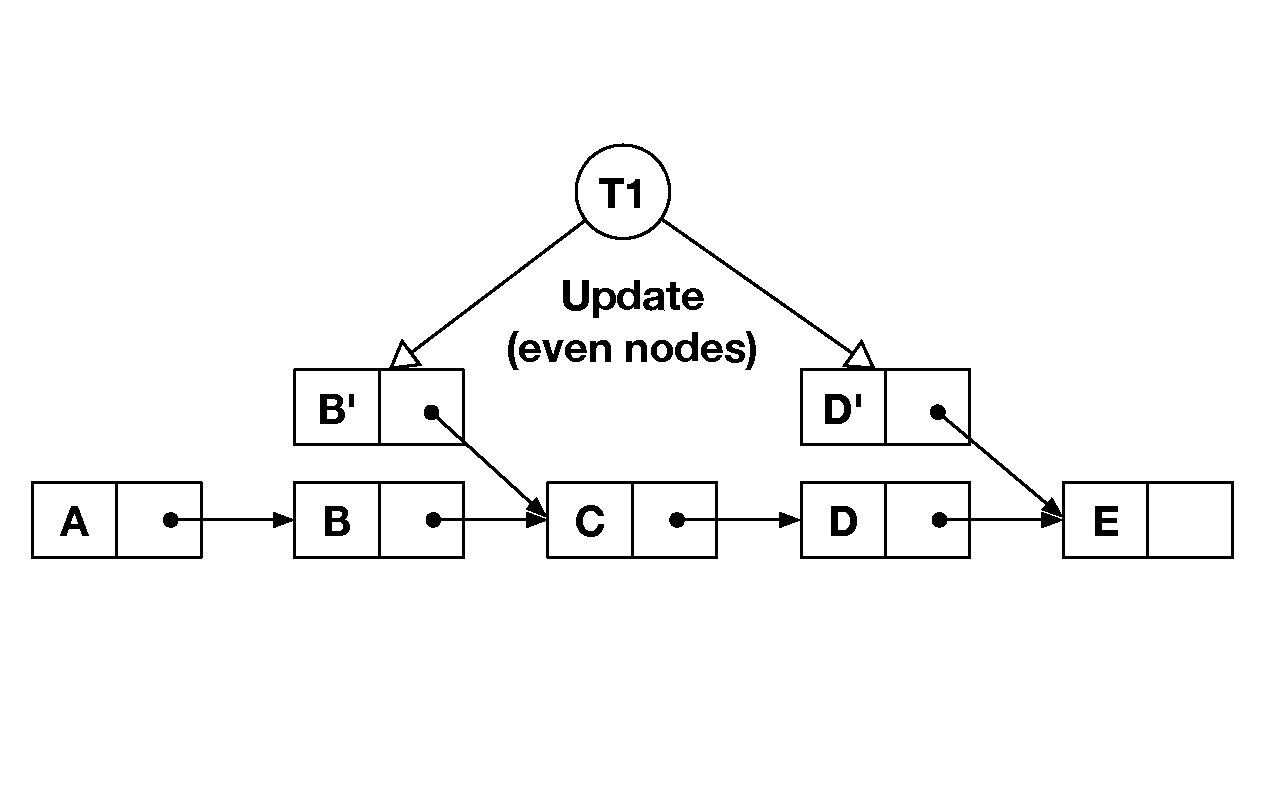
\includegraphics[width=1.0\textwidth]{figures/rcu_ex3}}
      \caption{Thread \emph{T1} wants to update all the even nodes. It
        traverses the list and create a duplicates for each node it wants to
        update.}
      \label{fig:rcu_ex3}
    \end{flushleft}
  \end{minipage}
  \hfill
  \begin{minipage}[t]{0.47\textwidth}
    \begin{flushright}
      \centering
      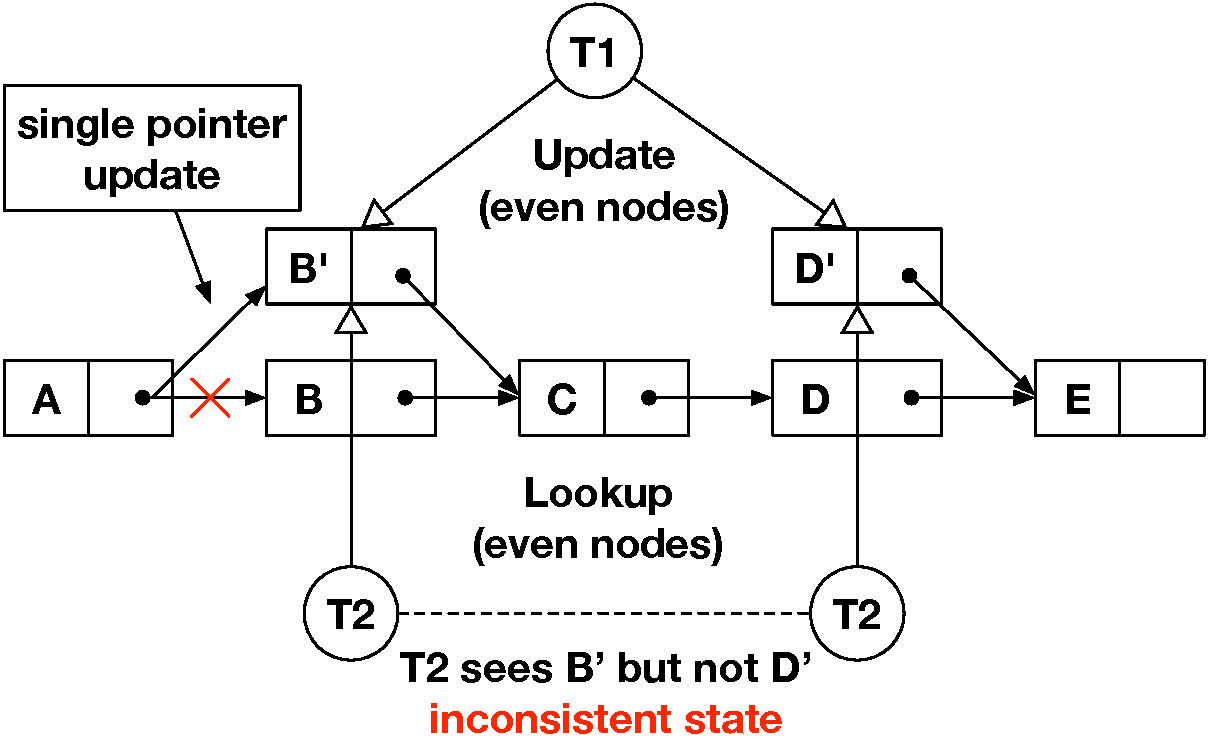
\includegraphics[width=1.0\textwidth]{figures/rcu_ex4}
      \caption{A second thread \emph{T2} wants to lookup for all the even
        nodes. RCU allows only single pointer updates, \emph{T1} cannot update
        the pointers to \emph{B'} and \emph{D'} simultaneously, so the thread
        \emph{T2} will see an inconsistent state.}
      \label{fig:rcu_ex4}
    \end{flushright}
  \end{minipage}
  \vspace{-5pt}
\end{figure}

\subsubsection*{RLU Description}
\label{sec:member412}
As stated above, RLU is an extension to RCU that provides both unsynchronized
traversal and multi-location atomic updates, simplifying the work of the
programmer but still guaranteeing efficiency and performance.
%
RLU allows multiple object updates in a single operation by combining RCU
mechanism with a global clock (inspired by TM mechanisms) and per-thread
object-level logs.

Specifically, RLU maintains different information (metadata) as global,
\mbox{per-thread} and \mbox{per-object}:

\paragraph{Global:} The only global information maintained by RLU are the
global clock, and a global array of threads used to determine the currently
active threads.

\vspace{-10pt}
\paragraph{Per-Thread:} Each thread maintains:

\begin{itemize}
\item two \emph{write-logs}: hold new object copies, each object in the
  write-log has a header that holds information such as: thread id, pointer to
  the actual object in memory, object size.
\item \emph{local clock} (\emph{l-clock}) and \emph{write clock}
  (\emph{w-clock}): control the write-log stealing mechanism of threads.
\item \emph{run counter}: indicates when the thread is active.
\end{itemize}

\vspace{-10pt}
\paragraph{Per-Object:} RLU attaches to each object a header which contains a
pointer to the copy of the object in a write-log (\emph{malloc()} calls are
hooked with a call to a \emph{rlu\_alloc()} function that attaches the header
at the object allocation time).
%
When there is no copy the pointer is \emph{NULL}.
%
RLU API provides specific macros and functions to access and modify the
metadata headers of an object.
\\

\noindent
The RLU algorithm works approximately in the following way:

\begin{itemize}
\item When an operation starts (read or write), it always reads the global
  clock first.
\item Each write operation that wants to modify a shared object, first copies
  the object in a per thread write-log and modifies the copy.
\item A write operation locks the object at its first modification (and
  duplication) in order to avoid conflicts with concurrent writes.
\item Each thread maintains a local clock (\emph{l-lock}) that reflects the
  value of the global clock (\emph{g-lock}), and a write clock
  (\emph{w-clock}, initially initialized to $\infty$) that is used by a thread
  to determine whether it needs to steal a new object copy (from a writing
  thread) or can read it from memory.
  %
  Therefore, when a thread wants to read an object:
  \begin{itemize}
  \item If it is not locked (by a thread $T_w$ performing a write operation)
    reads it from memory.
  \item If it is locked:
    \begin{itemize}
    \item If \emph{l-clock} $\geq T_w$.\emph{w-clock} steals the new copy from $T_w$.
    \item Read the object from memory, otherwise.
    \end{itemize}
  \end{itemize}
\item To commit the new object copies, a write operation computes the new
  clock value and stores it into the \emph{w-clock}, \emph{l-clock}, and
  \emph{g-clock} in this order.
  %
  The update of the clock divides the operations into two categories:
  \begin{itemize}
  \item \emph{old operations}, those that started before the clock update.
    %
    These operations will read the old object copies.
  \item \emph{new operations}, those that started after the clock update.
    %
    These operations will read the new object copies from the writer.
  \end{itemize}
  %
  The writer waits until \emph{old operations} have finished (\emph{grace
    period}, this wait is implemented by calling the \emph{RLU\_SYNCHRONIZE}
  function), and then it can safely overwrite the old objects in memory with
  the new objects from the writer-log.
  %
  It releases the locks.
  \item The basic algorithm does not provide write--write synchronization which must
    be managed by the programmer.
    %
    An easy approach to synchronize multiple write operations is to execute them
    serially.
\end{itemize}

% RLU provides a simple synchronization mechanism that is comparable and
% sometimes better in terms of performance than RCU and it simplify programmers
% work presence of race conditions.

\paragraph{Example:}

\begin{figure}[t]
  \begin{minipage}[b]{0.47\textwidth}
    \begin{flushleft}
      \centering
      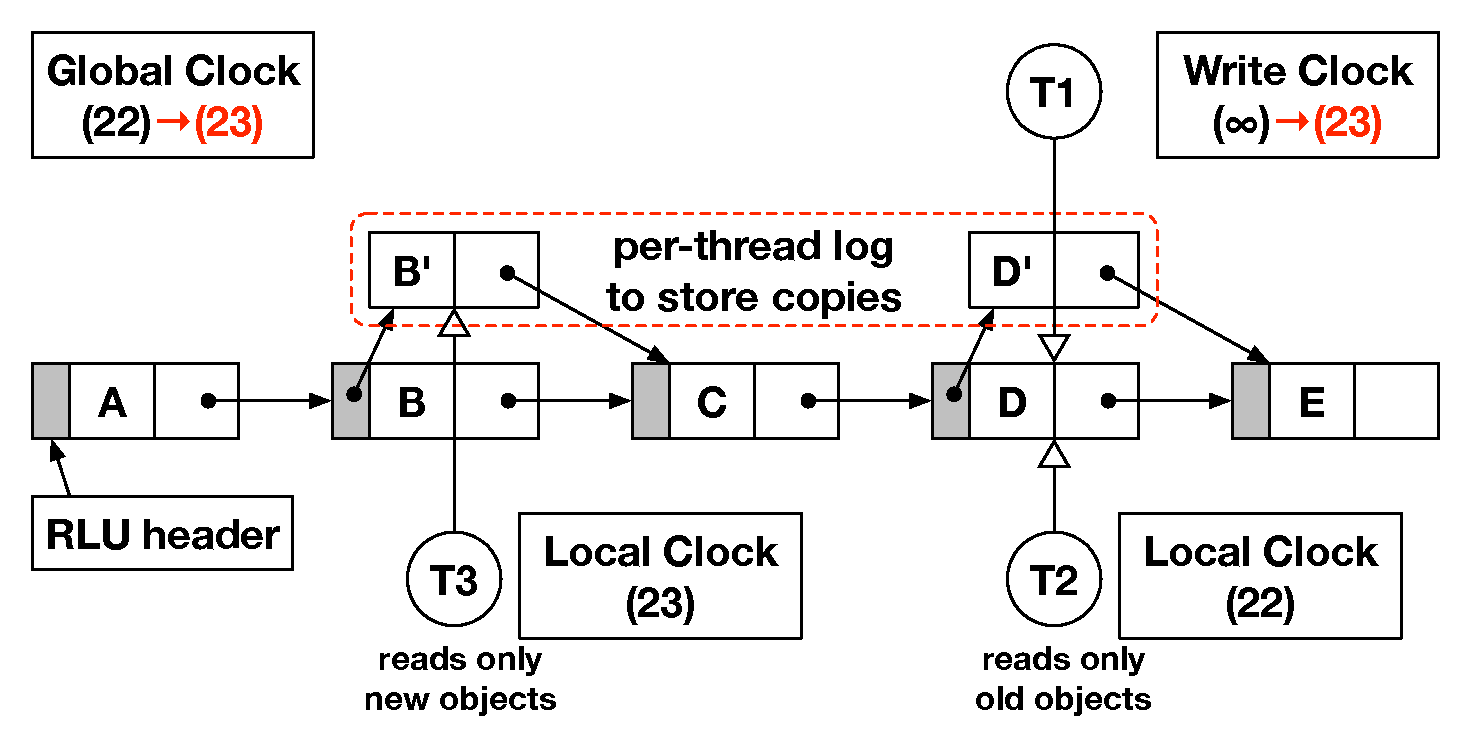
\includegraphics[width=1.0\textwidth]{figures/rlu_ex1}
      \caption{Thread $T1$ copies the object ``B'' and ``D'' in the per-thread
        write-log, updates the values and start the commit procedure by
        updating the clocks (in red). Thread $T2$ (that started the operation
        before the commit) reads the object ``D'' from the memory, while
        thread $T3$ (that started the operation before the commit) reads the
        object ``B'' from the $T1$'s per-thread write-log.}
      \label{fig:rlu_ex1}
    \end{flushleft}
  \end{minipage}
  \hfill
  \begin{minipage}[b]{0.47\textwidth}
    \begin{flushright}
      \centering
      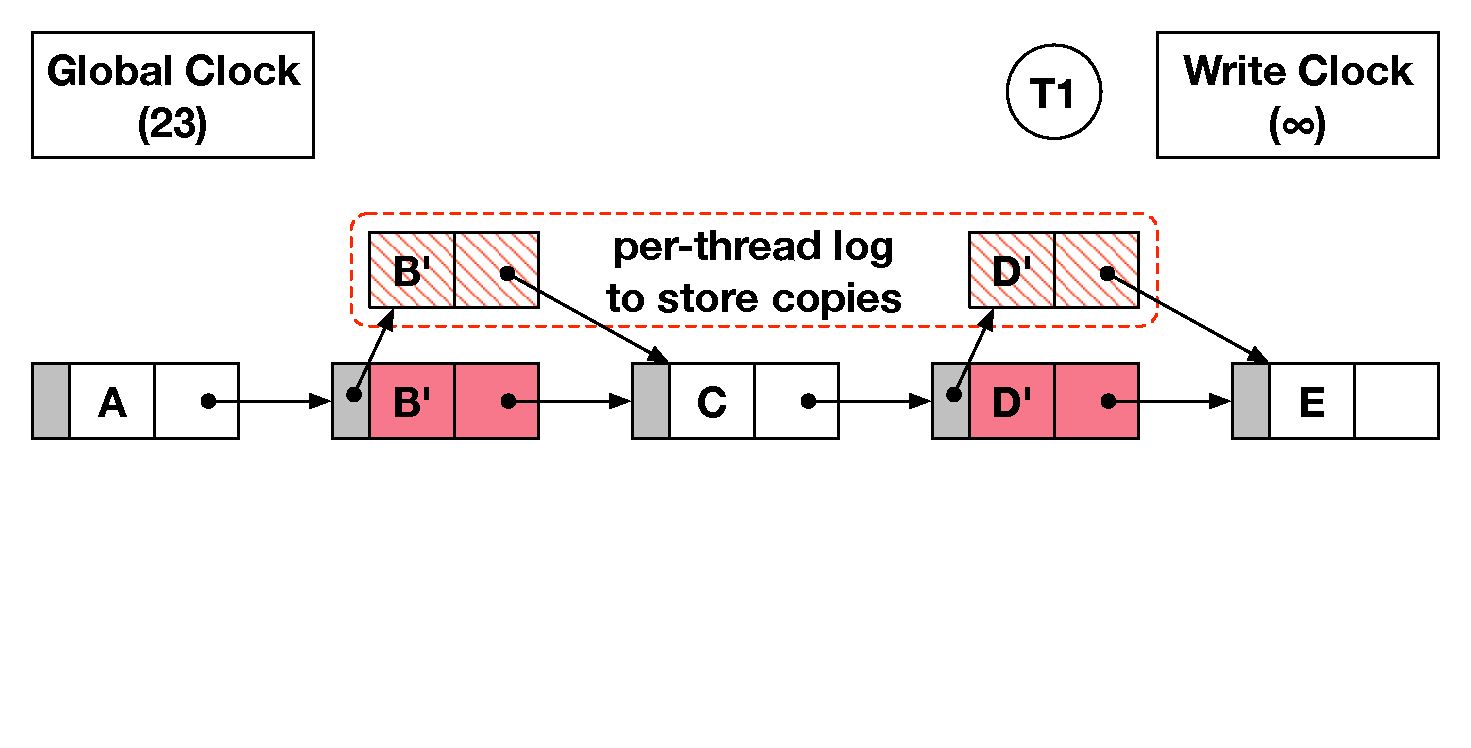
\includegraphics[width=1.0\textwidth]{figures/rlu_ex2}
      \caption{Thread $T1$ writes the modification in memory, swaps the log
        and reset the write-clock to $\infty$. \textcolor{white}{empty empty
          empty empty empty empty empty empty empty empty empty empty empty
          empty empty empty empty empty empty empty empty empty empty empty
          empty empty empty empty empty empty empty empty empty empty empty}}
      \label{fig:rlu_ex2}
    \end{flushright}
  \end{minipage}
  \vspace{-10pt}
\end{figure}

Figure~\ref{fig:rlu_ex1} and Figure~\ref{fig:rlu_ex2} show an example of RLU
algorithm.
%
Each object has a header that contains the pointer to the object copy in the
write-log of a thread, initially the pointer is \emph{NULL}.
%
When a thread $T1$ wants to modify some objects (e.g.\ nodes $B,D$), it first
tries to lock the objects, and if successful, generates the copies, storing
them in the per-thread write-log.
%
A second thread $T2$ that wants to read an object, first updates its local
clock to the value of the global clock.
%
The local clock is used by the reading thread to decide if it has to read the
real object from memory or the copy of the object from some per-thread
write-log.
%
The writer instead has a write clock which is initialized to $\infty$.
%
Whenever $T1$ wants to commit its modifications, it first updates the clocks:
write clock and global clock to the next value (from $22$ to $23$ in
Figure~\ref{fig:rlu_ex1}).
%
At this point, the old copies are reachable by the threads that started
reading the objects before the global clock update, while the new copies are
reachable by the thread that started after the global clock update.
%
Thread $T2$ will keep seeing the old copies, while $T3$ will see the new
copies, as in Figure~\ref{fig:rlu_ex1}.
%
The threads make a simple check, whenever their \emph{l-clock}
$\geq T_w$.\emph{w-clock} they steal the new copy from the per-thread
write-log of the writing thread, otherwise they read the old object from
memory.
%
In this case it is impossible for the threads to read a mix of state, as
happened in RCU, they will see either all the new object or all the old
objects.
%
In the next step of the commit $T1$ wait for the \emph{grace period} (calling
\emph{RLU\_SYNCHRONIZE}), to wait for the old reading threads ($T2$) to
finish.
%
When thread $T2$ is done, $T1$ writes the new objects back to memory
(Figure~\ref{fig:rlu_ex2}), resets the write clock to $\infty$, and unlock the
object.
%
It is important to notice that, it is necessary to wait for another
\emph{grace period} before clearing the current write-log and reusing it.
%
The reason for this is that it may still be used by threads that stole the
copies from this write-log.
%
Therefore, the writing thread, as a last operation of the commit, swaps the
\emph{current write-log} with a \emph{new write-log} (remember each thread has
two write-log available), and waits for the completion of the next
\emph{RLU\_SYNCHRONIZE} to swap again the logs and reuse safely the
\emph{current write-log}.

\subsection*{Explain the problem that RLU Deferring (Section 3.7) solves and
  give a pathological example scenario where RCU’s ``synchronize'' operation
  would have high overheads but RLU Deferral would not.}
\label{sec:member42}
\vspace{-5pt}
The RLU experiments show that when operations are short and fast, the
algorithm performance decreases significantly.
%
This is because every time a writer has to perform a write, it calls the
\emph{RLU\_SYNCHRONIZE} function, which implements the wait of the \emph{grace
  period} that a writer has to let pass to safely write the updated objects
back to memory.
%
The \emph{RLU\_SYNCHRONIZE} calls introduces a high overhead, i.e.\ for each
small write operation the writer has to wait the \emph{grace period}.
%
In order to solve this performance problem, the authors introduce a variant to
RLU called \emph{RLU Deferring}, that indeed defers (or delays) the call to
the \emph{RLU\_SYNCHRONIZE} as much as possible -- making this call only if
strictly necessary.

RLU Deferring works in the following way.
%
At each commit phase, after the writer stores the current write-log, it
generates a new one for the next write operation.
%
This allows to keep performing write operations without blocking until a
different thread needs to update an object that is already locked.
%
Only at this moment, the new writer issues a ``sync request'' to the writer
thread that is holding the lock in order to force it release the lock.
%
Therefore, the writer thread performs the normal operations: increment global
clock, execute the \emph{RLU\_SYNCHRONIZE} call, write the objects to memory
and finally unlock.

RLU Deferring introduces significant advantages in terms of performance, since
it heavily limits the number of actual write--write conflicts.
%
It also reduces the global clock updates, which as a consequence delays the
stealing process, allowing threads to read from memory (instead from a thread
write-log), and experience less or none cache misses (higher in number when
the memory is updated more often).
\\

An example that would show the advantages of RLU Deferring compared to RCU is
given by a benchmark where multiple threads perform a high rate of updates on
a linked-list while other threads read the same objects.
%
In RCU, when a thread updates an object, it has to commit (since it only
performs single-pointer updates), and let the \emph{grace period} pass prior
to starting the next write operation.
%
This is to wait for the reading threads to terminate their operations.

In RLU Deferring, the call to \emph{RLU\_SYNCHRONIZE} happens only when a
write--write conflict manifests.
%
In this case, the current writing thread receives the ``sync request'' from a
new writer, and it has to perform the commit and call the synchronize
function.
%
If no write--write conflict happens, the writing threads can keep updating the
objects while the reading threads access the copies.
%
RLU Deferring waits for a smaller number of \emph{grace periods} than RCU,
reducing the runtime overhead.

In general, increasing the number of writers (and so write--write conflicts)
RCU introduces a sequential bottleneck, while RLU Deferral can perform
concurrently the write operations increasing the scalability.
%
The authors in Figure~10 of~\cite{Matveev:2015:RLS:2815400.2815406} show the
best performance of RLU compared to RCU, increasing the updates rates on a
linked-list.
%
This should reinforce the fact that RLU Deferral (which is faster than RLU)
have less overheads than RCU, as described in the previous example.

However, the experimental results show that this optimization is more
significant for a high number of cores ($>20$).
%
Therefore, a better example that shows the performance boost of the deferring
approach is the benchmark on Citrus Tree on a 80 cores machine.
%
Indeed, the performance results show that for an high threads count RLU
Deferral is faster than RCU by a factor of two.
%
This is because RCU has to execute the synchronization call for each delete,
while RLU Deferral calls the synchronization function only on actual
write--write conflicts.

\subsection*{Can RLU Deferral result in linearizability violations?}
\label{sec:member43}
\vspace{-5pt}
RLU Deferral can not result in linearizability violations, because it
guarantees that when a thread commits a write operation all the other threads
that started later than the commit operation will see the value of that write.
%
When a thread performs a commit it first increments the global clock,
which splits the concurrent threads operations in \emph{old operations} and
\emph{new operations}.
%
The old operations are those ones that started before the clock updates, so
these threads will read the old value of the objects thanks to the
per-thread write-log that contains the copies.
%
Furthermore, the new operations that started after the clock update will read
the new values from the new per-thread write-log (via stealing).
%
The threads can make this decision by first reading the global clock and
comparing it with the writing thread write clock.
%
This allows a thread to ``understand'' if they started an operation before or
after the commit and so they should read the new or the old value.
%
If a write--write conflict happens, the writing thread receives a ``sync
request'' and besides executing the commit it also calls the
\emph{RLU\_SYNCHRONIZE}, that makes the writing thread wait for the \emph{old
  operations} to finish, prior to writing the updates on memory.
%
As the commit updated the global clock the new write operation will now see
the new value.
%
This guarantees that each thread is always able to see a consistent memory
state (that could happened in some serial execution) which existed at the
global time when it started the operation.

\subsection*{Does code using RLU Deferral in 3.7 meet the definition of being
  ``lock-free''?}
\label{sec:member44}

\vspace{-5pt}
Considering the definition of lock-free
in~\cite{Herlihy:2008:AMP:1734069}~\footnote{A method is lock-free if it
  guarantees that infinitely often some method call finishes in a finite
  number of steps.
  %
  Let us also consider some larger ADT lock-free if and only if all of the
  operations/methods on it are lock-free.}.
%
A code using RLU Deferral can be considered lock-free for read operations and
non lock-free for write operations.

\begin{itemize}
\item \emph{Read Operations}: Read operations are lock-free because a reading
  thread can always make progress and there is nothing that can stop them from
  proceeding.
  %
  A reading thread can always decide, based on the values of the global clock
  and the writer clock, to read an object from the memory (old value) or from
  a thread write-log (new value).
\item \emph{Write Operations}: Write operations are non lock-free because
  there exists a situation where a new writer may be stopped by another writer
  that fails to respond to a ``sync request''.
  %
  In such circumstances the current writer never completes the commit
  operation and never calls the synchronize function, preventing the new
  writer to start its operations, thus none of the threads finish their
  operation in a finite number of steps.
\end{itemize}

\vspace{-10pt}
\printbibliography

\end{refsection}

%%% Local Variables:
%%% mode: latex
%%% eval: (flyspell-mode 1)
%%% TeX-master: "root.tex"
%%% End:
